\documentclass[10pt]{article}
\usepackage{icmlko}

\icmlmeta{IP 파운데이션 월드모델}{128}{나오기 전에 얼마나 찾아봤나}{작품 바깥에서 온 첫 축 --- 노트 126과 127이 가리킨 자리에 실제로 축을 하나 만들어 넣었다}

\begin{document}

\twocolumn[
\icmlheader

\begin{abstract}
지난 두 노트가 서로 다른 길로 같은 곳을 가리켰다. 노트 126의 F8은 ``같은
자질에 비선형을 얹어도 안 오른다''(병목은 모형이 아니라 축)고 했고, 같은
노트의 F11은 ``한 도메인에만 있는 축은 도움이 안 된다''고 했다. 남는
처방은 하나 --- \textbf{전 도메인이 공유하는 새 축을 만든다.} 그래서
만들었다. \textbf{오픈 전 검색 관심도.} 네이버 데이터랩에서 작품이 나오기
\emph{이전} 창의 검색량을 앵커 정규화해 수준 · 모멘텀 · 변동성 · 정점비
넷으로 요약한다. 지금까지의 후보 축(설명문 임베딩 · 표지 특징 · 평점)은
전부 \emph{작품 자신의 메타데이터}였다 --- 이것은 처음으로 \textbf{작품
바깥의 수요 신호}다. 도메인 다섯을 새로 긁어 3{,}101행을 채웠다(요청 724회).
\textbf{신호가 세다.} 라벨과의 상관이 게임 $+$0.40 · 도서 $+$0.35 · 애니
$+$0.23 · 모바일 $+$0.20이고 모멘텀은 게임에서 $+$0.47이다. \textbf{그리고
새 정보다} --- 손으로 매긴 축 다섯과의 겹침이 대개 $|r|<0.25$이고, 손 축으로
맞춘 \emph{잔차}와의 상관이 원 상관과 거의 같다(게임 $+$0.25 · 도서 $+$0.29
· 모바일 $+$0.19). \textbf{하네스에서 검색 축 실행 여덟이 기본 실행 전부를
이긴다.} 판 $\rho$가 부스팅에서 $+$0.3363에서 \textbf{$+$0.4019}로 오르고
--- 이 판의 최고치다 --- 귀무 대비 $z$도 $+$4.41에서 $+$5.39로 오른다.
더 맞히면서 동시에 덜 유연해졌다. 여덟 실행 모두 가드 일곱을 통과한다.
\textbf{그런데 팝업은 내린다} --- 제품이 묻는 바로 그 자리다. 팝업의 검색어는 브랜드명이고
브랜드 인지도는 팝업 유입과 다른 것이라는 뜻으로 읽는다. 한계 둘을
적어 둔다. 만화 · 세계애니는 제목이 로마자뿐이라 한국어 검색이 안 붙어
\textbf{덮음 0}이고, 웹툰은 라벨이 네이버 즐겨찾기라 이 축과 \emph{같은
플랫폼}이어서 아예 안 긁었다(노트 117의 출처 차단).
\end{abstract}
]

\begin{figure*}[t]
\centering
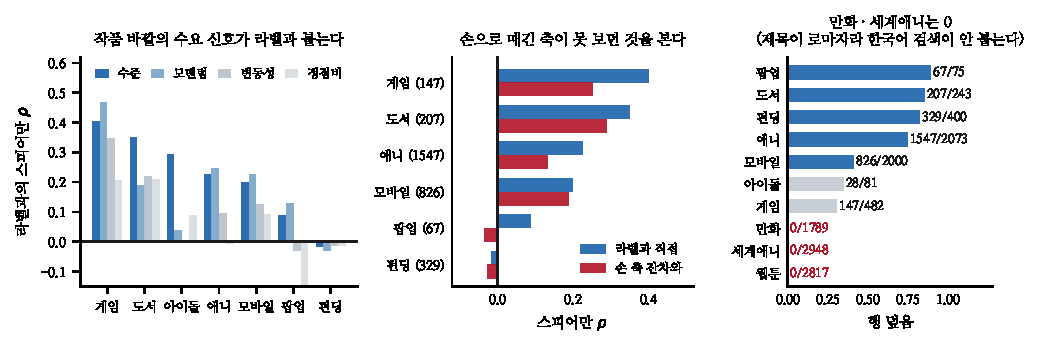
\includegraphics[width=\textwidth]{figs/trend.pdf}
\caption{왼쪽 --- 작품 바깥의 수요 신호가 라벨과 붙는다. 가운데 --- 손으로
매긴 축으로 맞춘 잔차와도 붙는다(새 정보다). 오른쪽 --- 도메인별 덮음.}
\end{figure*}

\section{두 노트가 같은 곳을 가리켰다}

노트 126은 도전자 일곱을 붙여 놓고 둘을 알아냈다. 하나는 F8 --- F6과
\emph{완전히 같은 자질}에 히스토그램 부스팅을 얹었는데 판 $\rho$가 오히려
내렸다($+$0.3413 $\to$ $+$0.3363). 모형을 바꿔서 얻을 것이 없다는 뜻이다.
다른 하나는 F11 --- 게임에만 있는 축 넷을 더했더니 판 $\rho$가 내리고
\emph{게임 자신이} $+$0.5473에서 $+$0.3798로 내렸다. 한 도메인의 이력으로만
정해지는 모수는 지평 너머에서 배신한다는 그 노트의 법칙이다.

둘을 겹치면 처방이 하나로 좁혀진다.

\claimx{\textbf{모형이 아니라 축을 늘려야 하고, 그 축은 전 도메인이 공유하는
것이어야 한다.} 노트 127이 그 처방으로 기획서 태거를 만들었지만 거기서
막혔다 --- 태거는 배운 종류의 레코드 안에서만 맞았다.}{``공유하는 축''이라는
조건은 노트 126의 관측 한 판에서 나온 것이다.}

\section{작품 바깥에서 축을 하나 가져온다}

지금까지 시험한 후보 축을 다시 보면 공통점이 있다. 설명문 임베딩 여덟 ·
글 길이 · 표지 밝기 · 평점 · 장르 수 --- \textbf{전부 작품 자신이 들고
있는 것}이다. 작품을 아무리 자세히 들여다봐도 ``세상이 이걸 얼마나
기다리고 있나''는 안 나온다.

네이버 데이터랩은 그것을 준다. 전 국민 검색을 덮고 2016년까지 소급되며
공식 API라 시점이 정확하다. 설계에서 두 가지가 중요하다.

\claimx{\textbf{앵커 정규화.} 데이터랩은 절대 검색량이 아니라 요청 묶음 안
최댓값을 100으로 둔 \emph{상대지수}를 준다. 그래서 서로 다른 요청의 값은
비교가 안 된다. 모든 요청에 고정 앵커(``날씨'')를 같이 넣고 대상/앵커
비율로 환산해야 작품 간 · 시점 간 비교가 성립한다.}{앵커 자체의 검색량이
장기 추세를 가지면 환산값이 휜다. ``날씨''는 계절성이 있지만 대상도 같은
계절을 겪으므로 비율에서는 상당 부분 상쇄된다 --- 정량화는 안 했다.}

\claimx{\textbf{창은 오픈 이전만.} 상태 특징은 오픈일 \emph{이전} 최대
12주에서만 계산한다. 그래서 시간 마스크를 자동으로 통과한다 --- 예측
시점에 실제로 알 수 있는 값이다.}{오픈일 자체가 틀린 레코드가 있으면
창도 틀린다. 도메인마다 발매일 · 출간일 · 연재시작일을 썼다.}

\begin{table}[t]
\centering\tsize
\caption{긁은 것. 요청 724회(일 한도 1,000).}
\begin{tabular}{lrr}
\toprule
& 덮인 행 & 덮음 \\
\midrule
팝업 & 67 / 75 & 89\% \\
도서 & 207 / 243 & 85\% \\
펀딩 & 329 / 400 & 82\% \\
애니 & 1{,}547 / 2{,}073 & 75\% \\
모바일 & 826 / 2{,}000 & 41\% \\
아이돌 & 28 / 81 & 35\% \\
게임 & 147 / 482 & 31\% \\
\midrule
만화 · 세계애니 & 0 & \textbf{0\%} \\
웹툰 & --- & 안 긁음 \\
\bottomrule
\end{tabular}
\end{table}

\section{신호가 있고, 새 정보다}

첫 질문은 ``라벨과 붙나''다. 붙는다 --- 그것도 세게.

\begin{table}[t]
\centering\tsize
\caption{검색 축과 라벨의 스피어만. 도메인 안에서 잰 것.}
\begin{tabular}{lrrr}
\toprule
& 수준 & 모멘텀 & $n$ \\
\midrule
게임 & $+$0.402 & $+$0.468 & 147 \\
도서 & $+$0.350 & $+$0.189 & 207 \\
아이돌 & $+$0.292 & $+$0.038 & 28 \\
애니 & $+$0.226 & $+$0.247 & 1{,}547 \\
모바일 & $+$0.200 & $+$0.226 & 826 \\
팝업 & $+$0.088 & $+$0.130 & 67 \\
펀딩 & $-$0.014 & $-$0.029 & 329 \\
\bottomrule
\end{tabular}
\end{table}

두 번째 질문이 더 중요하다. \emph{손으로 매긴 축이 이미 잡고 있던 것을
다시 잡는 것뿐인가?}

\claimx{\textbf{아니다. 새 정보다.} 검색 축과 손 축 다섯의 겹침은 대개
$|r|<0.25$이고(가장 큰 것이 게임의 굿즈 규모 $+$0.495), 손 축으로 맞춘
\emph{잔차}와의 상관이 원 상관과 거의 같다 --- 게임 $+$0.402가 잔차에서
$+$0.253, 도서 $+$0.350이 $+$0.289, 모바일 $+$0.199가 $+$0.187이다.}{팝업과
펀딩은 잔차 상관이 0 이하다 --- 이 축이 아무것도 안 더한다.}

\section{하네스 --- 여덟이 전부 이긴다}

축 세트를 자료 쪽에 두고(정식화마다 ``+검색'' 변형을 만들지 않는다) 네
정식화를 세 세트로 돌렸다. 대상 집합은 셋 다 같다 --- 축을 더해도 행은
안 변하므로 분모 규칙(노트 82 · 90)이 자동으로 지켜진다.

\begin{table}[t]
\centering\tsize
\caption{판 $\rho$ · 배포 규약 $T$=2025.0. 가드 일곱 전부 통과.
\texttt{trend}는 빈 계열을 0으로, \texttt{trend0}은 결측으로 본다.}
\begin{tabular}{lrrrr}
\toprule
& 공통 다섯 & $+$검색 & $+$검색$_0$ & $z$ \\
\midrule
F8 부스팅 & $+$.3363 & \textbf{$+$.4019} & $+$.3890 & $+$5.39 \\
F10 도메인별 수축 & $+$.3452 & $+$.3872 & $+$.3961 & $+$4.27 \\
F9 짝 순위 우도 & $+$.3464 & $+$.3736 & $+$.3843 & $+$3.41 \\
F6 직접 풀링 & $+$.3413 & $+$.3704 & $+$.3793 & $+$3.58 \\
\bottomrule
\end{tabular}
\end{table}

\claimx{\textbf{축 하나가 모형 일곱보다 컸다.} 노트 125부터 127까지 정식화를
일곱 붙여 얻은 최대 폭이 $+$0.013(F6 $\to$ F2)이었다. 축 넷을 더한 이번
폭은 $+$0.027$\sim$$+$0.066이다. F8이 제일 크게 오른 것이 특히 말이 된다
--- 그 정식화가 바로 ``병목은 축''을 진단한 도구였고, 축이 오자 비선형이
비로소 값을 한다.}{한 시간 분할 한 판이다. 그리고 덮음이 도메인마다 크게
달라(31\%$\sim$89\%) 이득의 배분이 덮음에 끌린다.}

\claimx{\textbf{귀무 폭도 같이 줄었다.} F6이 0.1266에서 0.1067로, F9가
0.1348에서 0.1123으로, F10이 0.1120에서 0.0926으로 좁아졌다. 더 맞히면서
동시에 덜 유연해진 것이다 --- 노트 126의 법칙이 경계하던 방향과 반대다.
전 도메인 공통 축이라 한 도메인의 표류에 덜 노출된다.}{귀무는 치환 99회로
잰 것이라 폭 자체에도 오차가 있다.}

\claimx{\textbf{0을 측정값으로 볼지 결측으로 볼지는 안 갈렸다.} 논리는 0
쪽이 맞는데(물어봤더니 아무도 안 찾았다) 실측은 F8만 \texttt{trend}가 낫고
나머지 셋은 \texttt{trend0}이 낫다. \textbf{그래서 고르지 않았다} --- 둘 다
축 세트로 올려 두고 다음 분할에서 다시 잰다.}{바깥 점수를 보고 골랐다면
그게 노트 126이 잡은 바로 그 잘못이다.}

\section{누수는 두 층 다 통과한다}

노트 117이 라벨 누수로 두 번 뒤집힌 뒤 세운 규약이 둘이다.

\begin{table}[t]
\centering\tsize
\caption{누수 가드.}
\begin{tabular}{lll}
\toprule
& 문턱 & 결과 \\
\midrule
라벨 상관 & $|r|\ge$0.70 차단 & 최대 0.468 (통과) \\
출처 차단 & 라벨 만든 플랫폼 & 아래 참고 \\
\bottomrule
\end{tabular}
\end{table}

출처를 하나씩 보면 --- 모바일 라벨은 앱스토어 평점 수, 도서는 알라딘
판매지수, 게임은 스팀, 아이돌은 초동 음반 판매, 팝업은 현장 방문자다.
어느 것도 네이버가 아니다.

\claimx{\textbf{웹툰만 걸린다.} 웹툰 라벨은 네이버 웹툰 즐겨찾기이고 이
축은 네이버 검색이다. 같은 플랫폼의 다른 계수기라 노트 119--121이 잰
결합(자기 $\rho$의 21$\sim$38\%가 부풀림)이 그대로 걸릴 수 있다. 그래서
\textbf{아예 안 긁었다.}}{웹툰은 후행 표본이 711건으로 제일 큰 대상이다.
그걸 빼고 재는 것이니 이번 이득은 웹툰 몫이 빠진 값이다.}

\section{팝업은 내린다}

하네스 결과에서 하나가 눈에 걸린다. 판 전체는 오르는데 \textbf{팝업은
내린다.} 제품이 묻는 바로 그 자리다.

대상별로 보면 아이돌 $+$0.138 · 모바일 $+$0.121 · 도서 $+$0.112 · 애니
$+$0.045로 오르고, 게임 $-$0.136 · 팝업 $-$0.045 · 펀딩 $-$0.020으로 내린다.
판이 오르는 것은 오르는 쪽 표본이 더 크기 때문이다(모바일 441 · 애니 606
대 게임 223).

\claimx{\textbf{게임이 제일 크게 내린다 --- 덮음이 31\%뿐이다.} 라벨과의
상관은 게임이 $+$0.402로 제일 높은데 그 값을 아는 행이 셋 중 하나다.
나머지 셋 중 둘은 중립 대입을 받고, 모형은 ``검색량이 높다''와 ``검색량을
모른다''를 같이 배워야 한다.}{덮음과 이득의 관계는 도메인 일곱의 상관이지
인과가 아니다. 게임 덮음을 올려 보면 갈린다 --- 게임 제목의 67\%가
로마자라 한계가 있다.}

\claimx{\textbf{팝업의 검색어는 브랜드명이지 팝업 이름이 아니다.} 수집기가
쓰는 키는 \texttt{brand\_key}(예: ``폴햄'')이고, 그건 브랜드 인지도를
잰다. 팝업 유입은 브랜드 인지도와 다른 것 --- 이미 유명한 브랜드가 작은
팝업을 열기도 하고 무명 IP가 줄을 세우기도 한다. 잔차 상관 $-$0.034가
그 말을 한다.}{``브랜드 인지도''와 ``팝업 유입''이 다르다는 것은 해석이지
측정이 아니다. 팝업 이름 자체로 다시 긁어 보면 갈린다 --- 다만 팝업 이름은
오픈 이전에 검색되지 않는 경우가 많아 창이 비게 된다.}

\section{수집에서 배운 것 둘}

\claimx{\textbf{하나 --- 물어봤는데 없는 것은 결측이 아니라 0이다.}
데이터랩이 빈 계열을 주는 경우가 물어본 것의 45\%(1{,}151건)다. 처음엔
결측으로 읽어 마스크를 내렸는데, 그건 ``아무도 안 찾았다''를 통째로
버리는 것이다. 창이 오픈 210일 전부터라 계열이 오기만 하면 점이 반드시
넷 이상 나오므로, 빈 계열은 곧 검색량이 보고 문턱 아래라는 뜻이다.}{논리는
0 쪽이 맞는데 \emph{하네스에서는 살짝 낮게 나왔다}. 그래서 어느 쪽도
고르지 않고 축 세트 둘(\texttt{trend} · \texttt{trend0})로 나란히 올려
가드에 맡겼다 --- 바깥 점수를 보고 고르면 노트 126이 잡은 그 잘못이다.}

\claimx{\textbf{둘 --- 검색량은 작품의 성질이지 레코드의 성질이 아니다.}
수집기는 같은 검색어를 두 번 사지 않으려고 키워드로 중복을 없앴고, 그래서
값이 그 키워드를 처음 쓴 레코드 하나에만 남았다. 읽을 때 키워드로 펴
주자 도서 덮음이 24\%에서 42\%로 올랐다(재수집 0회).}{같은 제목의 다른
작품은 같은 값을 받는다 --- 동명이인 문제는 안 풀었다.}

\section{남은 것}

\begin{table}[t]
\centering\tsize
\caption{다음.}
\begin{tabular}{ll}
\toprule
웹툰 & 같은 플랫폼 결합을 실제로 재고 나서 결정 \\
만화 · 세계애니 & 한국어 제목 매핑(AniList 동의어 · 라프텔) \\
팝업 & 브랜드명 말고 팝업 이름으로 다시 \\
펀딩 & 프로젝트명 말고 창작자명으로 \\
\bottomrule
\end{tabular}
\end{table}

덮음이 제일 낮은 곳이 제일 큰 대상이다. 웹툰(711) · 모바일(441)이 각각
0\%와 41\%다. 이 축의 값어치는 아직 절반도 안 쓴 셈이다.

\end{document}
